\chapter{ЛИТЕРАТУРНЫЙ ОБЗОР}

\section{Мониторинг электрических сетей}

Система \textbf{АСКУЭ --- Автоматизированная Система Коммерческого Учета Электроэнергии}, направлена на обеспечение контроля работы всего энергетического оборудования, а также комплексный и одновременно технический учет электроэнергии. Данная система разработана в целях применения на промышленных предприятиях, электростанциях и снабжающих электроэнергией организациях. В основе построения данной системы лежит связь счетчика-коммуникатора с другими подключенными к нему счетчиками, а также непосредственно с центрально управляющим сервером, который принимает всю информацию, идущую от счетчиков. Большим плюсом данной системы является то, что счетчик-коммуникатор заменил собой многие устройства, используемые до этого \cite{ascaepinfo}.

АСКУЭ является является специальной системой автоматизированного управления электроснабжением, в состав которой входят только информационные функции, а именно:
\begin{itemize}
\item централизованный контроль и измерение технологических параметров электроснабжения;
\item косвенное измерение параметров электроснабжения (технико-экономических показателей, внутренних переменных);
\item обощенная оценка и прогноз состояния автоматизированного технологического комплекса и его оборудования;
\item подготовка и передача данных в смежные и вышестоящие системы управления (бухгалтерия, плановый отдел);
\item удаленное управление объектами электроэнергохозяйства; формирование и выдача
данных оперативному персоналу;
\end{itemize}

Статегические цели содержания системы:
\begin{itemize}
\item повышение оперативности работы с заказчиками;
\item своевременное выявление спорных ситуаций;
\item целенаправленное ведение процесса энергоснабжения и обеспечения смежных и вышестоящих систем управления оперативной и достоверной информацией;
\end{itemize}

\section{Технологии передачи данных}

Существует множество различных технологии передачи данных, которые могут использоваться в УСПД. Каждая технология имеет свои достоинства и недостатки. Поскольку заранее не известно в каких условиях будет эксплуатироваться УСПД, необходимо комбинировать различные технологии передачи данных в одном устройстве. Таким образом можно добиться повышенной надежности работы с точки зрения доставки данных до сервера. Существует две большие категории технологии передачи данных, которые различаются средой передачи, а именно:
\begin{itemize}
\item проводные;
\item беспроводные
\end{itemize}

\subsection{Семейство проводных технологий Ethernet}

\textbf{Ethernet} (от лат. aether --- эфир) ~--- пакетная технология передачи данных преимущественно локальных компьютерных сетей. Стандарты Ethernet определяют проводные соединения и электрические сигналы на физическом уровне, формат кадров и протоколы управления доступом к среде — на канальном уровне модели OSI. Ethernet в основном описывается стандартами IEEE группы 802.3. Ethernet стал самой распространённой технологией ЛВС в середине 90-х годов прошлого века, вытеснив такие устаревшие технологии, как Arcnet, FDDI и Token ring\cite{ethernetinfo}.

В зависимости от скорости передачи данных и передающей среды существует несколько вариантов технологии. Независимо от способа передачи стек сетевого протокола и программы работают одинаково практически во всех перечисленных вариантах. Рассмотрим лишь небольшую часть модификации (таблица \ref{ethernettable}), которые могут быть потенциально применены для данной работы:

\begin{table}[h!]
\caption{Разновидности модификации стандарта Ethernet \cite{ethersite2}}
\label{ethernettable}
\begin{tabular}{|c|m{30mm}|p{90mm}|}
\hline
Модификация & Пропускная способность & Описание\\
\hline
10BASE-T & 10 Мбит/с & Для передачи данных используется 4 провода кабеля витой пары (две скрученные пары) категории-3 или категории-5. Максимальная длина сегмента 100 метров.\\
\hline
100BASE-TX & 100 Мбит/с & Задействована витая пара категории 5, фактически используются только две неэкранированные пары проводников, поддерживается дуплексная передача данных, расстояние до 100 м.\\
\hline
100BASE-T2 & 100 Мбит/с & Cтандарт, использующий витую пару категории 3. Задействованы только две пары проводников. Поддерживается полный дуплекс, когда сигналы распространяются в противоположных направлениях по каждой паре. Скорость передачи в одном направлении — 50 Мбит/с.\\
\hline
100BASE-T4 & 100 Мбит/с & Cтандарт, использующий витую пару категории 3. Задействованы все четыре пары проводников, передача данных идёт в полудуплексе.\\
\hline
1000BASE-T & 1000 Мбит/с & Стандарт, использующий витую пару категорий 5e. В передаче данных участвуют 4 пары. Скорость передачи данных — 250 Мбит/с по одной паре. Используется метод кодирования PAM5, частота основной гармоники 62,5 МГц. Расстояние до 100 метров\\
\hline
\end{tabular}
\end{table}

%\begin{itemize}
%\item 10BASE-T, IEEE 802.3i --- для передачи данных используется 4 провода кабеля витой пары (две скрученные пары) категории-3 или категории-5. Максимальная длина сегмента 100 метров.;
%\end{itemize}

\newpage

\subsection{Система мобильной связи GSM}

\textbf{GSM} (от названия группы \textit{Groupe Special Mobile}, позже переименован в Global System for Mobile Communications) ~--- глобальный стандарт цифровой мобильной сотовой связи, с разделением каналов времени (TDMA) и частоте (FDMA)\cite{gsmwiki}.

В стандарте определены 4 диапазона частот: 850 МГц, 900 МГц, 1800 МГц, 1900 МГц. В Европе и Азии используется два диапазона: 900 и 1800 МГц. Сравнительная характеристика представлена в таблице \ref{gsmtable}.

\begin{table}[h!]
\caption{характеристика диапазонов GSM, используемых в Европе и Азии\cite{gsmchar}}
\label{gsmtable}
	\begin{tabular}{|m{70mm}|m{40mm}|m{40mm}|}
	\hline
	Характеристики & GSM-900 & GSM-1800\\
	\hline
	Рабочий диапазон BTS-MS, МГц & 935-960 & 1805-1880\\
	\hline
	Рабочий диапазон MS-BTS, МГц & 890-915 & 1710-1785\\
	\hline
	Ширина радиоканала, кГц & $200*2$ & $30*2$\\
	\hline
	Макс. мощность MS, Вт & 0,8-8 & 0,25-4 \\
	\hline
	\end{tabular}
\end{table}

GSM обеспечивает поддержку следующих услуг:
\begin{itemize}
\item услуги передачи данных (синхронный и асинхронный обмен данными, в том числе пакетная передача данных — GPRS);
\item передача речевой информации;
\item передача коротких сообщений (SMS);
\item передача факсимильных сообщений;
\end{itemize}

\newpage

\subsection{Wi-Fi}

В качестве еще одной технологии обмена данными между разрабатываемым контроллером и удаленным сервером, была выбрана технология беспроводных сетей на базе стандарта IEEE 802.11. Использование данной технологии в УСПД значительно расширяет область размещения устройства в здании, а значит, повышает гибкость системы в целом.

\textbf{Wi-Fi} является торговой марки Wi-Fi Alliance. Аббревиатура Wi-Fi произошла от английского словосочетания Wireless Fidelity, которое переводится как <<беспроводное качество>> или <<беспроводная точность>>. В настоящее время развивается целое семейство стандартов передачи цифровых потоков данных по радиоканалам.

IEEE 802.11n – самый передовой коммерческий WiFi-стандарт, на данный момент, официально разрешенный к ввозу и применению на территории РФ. В 802.11n используются частотные каналы в частотных спектрах WiFi 2.4GHz и 5GHz. Совместим с 11b/11a/11g. Хотя рекомендуется строить сети с ориентацией только на 802.11n, т.к. требуется конфигурирование специальных защитных режимов при необходимости обратной совместимости с устаревшими стандартами\cite{wifistandarts}.

Сам стандарт WiFi 802.11n вышел 11 сентября 2009 года.
Поддерживаются частотные каналы WiFi шириной 20MHz и 40MHz (2x20MHz).
Используемая радиочастотная технология: OFDM.
Используется технология OFDM MIMO (Multiple Input Multiple Output) вплоть до уровня 4х4 (4хПередатчика и 4хПриемника). При этом минимум 2хПередатчика на Точку Доступа и 1хПередатчик на пользовательское устройство.

В данной работе предполагается, что с помощью Wi-Fi соединения можно будет получать данные от разрабатываемого контроллера на мобильные устройства, в тех местах, где проводное соединение отсутствует. Также рассматривается возможность использовани местных беспроводных корпоративных сетей для отправки пакетов на сервер по сети Интернет.

\newpage

\section{Многофункциональный трехфазный счетчик электрической энергии <<Меркурий 230 ART-03>>}

<<Меркурий 230>> относится к электронным (цифровым) счетчикам электроэнергии. В таких счетчиках на вход измерительного элемента поступает переменный ток и напряжение для получения на выходе импульсов, число которых пропорционально измеряемой активной энергии. В качестве счетного механизма служит электронное или электромеханическое устройство, которое включает в себя дисплей и запоминающее устройство\cite{mercinfo1}. 

«Меркурий 230» используется для учета энергии (активной, реактивной) и мощности в трехфазных сетях переменного тока. Учет может проходить в одном или двух направлениях в трех или четырех проводных сетях с частотой 50 Гц с использованием измерительных трансформаторов или непосредственно с возможностью тарифного учёта по зонам суток, учёта потерь и передачи измерений и накопленной информации об энергопотреблении по цифровым интерфейсным каналам\cite{mercinfo2}.

\begin{figure}[h]
	\label{mercury}
	\centering
		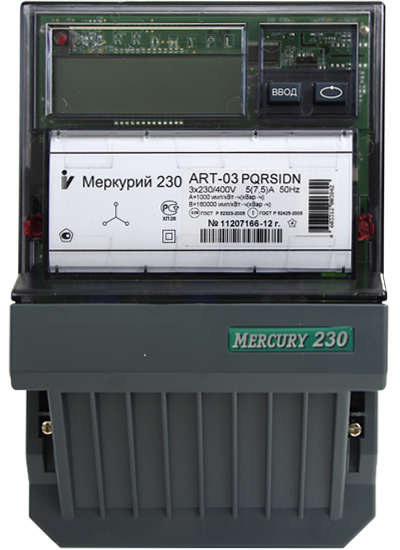
\includegraphics[scale=0.6]{img/mercury.png}
	\caption{<<Меркурий 230 ART-03>>}
\end{figure}

\newpage

\section{Протоколы}

Набор правил, позволяющий осуществлять соединение и обмен данными межджу двумя и более включёнными в сеть компьютерами, называется \textbf{сетевым протолом}.
Сами протоколы лишь описывают разные стороны одной и той же связи; взятые вместе, они образуют так называемый стек протоколов. Названия <<протокол>> и <<стек протоколов>> также указывают на программное обеспечение, которым реализуется протокол\cite{protocols}.

Распространённой системой классификации сетевых протоколов является так называемая модель OSI. В соответствии с этой моделью протоколы делятся на 7 уровней по своему назначению ~--- от физического до прикладного (см. таблицу~\ref{osi}). 

Протоколы работают друг с другом в стеке --- это означает, что протокол располагающийся на уровне выше, инкапсулируется в протокол нижнего уровня. Например, протокол UDP работает поверх протокола IP.

\begin{table}[h!]
\caption{Уровни протоколов в модели OSI}
\label{osi}
	\begin{tabular}{|c| >{\centering} m{120mm} <{\centering}|}
	\hline
	Уровень & Назначение \\
	\tabularnewline
	\hline
	Прикладной & Обеспечивает взаимодействие сети и пользователя. Уровень разрешает приложениям пользователя доступ к сетевым службам.\\
	\tabularnewline
	\hline
	Представления & Отвечает за преобразование протоколов и кодирование/декодирование данных.\\
	\tabularnewline
	\hline	
	Сеансовый & Отвечает за поддержание сеанса связи, что позволяет приложениям взаимодействовать друг с другом длительное время.\\
	\tabularnewline
	\hline
	Транспортный & Доставка данных без ошибок, потерь, дублирования и в правильной последовательности.\\
	\tabularnewline
	\hline
	Сетевой & Определение пути передачи данных. Нахождение кратчайших маршрутов.\\
	\tabularnewline
	\hline
	Канальный & Обеспечание взаимодействия сетей на физическом уровне и контроля за ошибками, которые могут возникнуть.\\
	\tabularnewline
	\hline
	Физический & Непосредственная передача потока данных через физическую среду.\\
	\tabularnewline
	\hline 
	\end{tabular}
\end{table}

\subsection{Стек протоколов TCP/IP}

\textit{Transmission Control Protocol/Internet Protocol (TCP/IP)} - это промышленный стандарт стека протоколов, разработанный для глобальных сетей\cite{tcpip}.

Этот стек протоколов был разработан до появления модели взаимодействия открытых систем. Несмотря на то, что он также имеет многоуровневую структуру, соответствие уровней стека TCP/IP уровням модели OSI весьма условно.

Работа УСПД напрямую зависит от способности поддерживать данный стек протоколов. Это объясняется следующим:
\begin{itemize}
\item Это метод получения доступа к сети Internet.
\item Это наиболее популярный и в то же время завершенный стандартный стек сетевых протоколов, имеющий многолетнюю историю
\item Все современные операционные системы поддерживают стек TCP/IP. 
\item Это устойчивая масштабируемая межплатформенная среда для приложений клиент-сервер.
\end{itemize}

Описание уровней и их назначения для стека протоколов TCP/IP можно посмотреть в таблице \ref{tcpiptable}.

\begin{table}[h!]
\caption{Стек протоколов TCP/IP}
\label{tcpiptable}
	\begin{tabular}{|c| >{\centering} m{100mm} <{\centering}|}
	\hline
	Уровень & Описание \\
	\tabularnewline
	\hline
	Прикладной & Обеспечивает взаимодействие сети и пользователя. За долгие годы использования накопилось обширное множество протоколов и сервисов прикладного уровня. Например: HTTP, FTP, SMTP, Telnet и множество других.\\
	\tabularnewline
	\hline
	Транспортный & На этом уровне функционируют два протокола. TCP и UDP. TCP обеспечивает надежную передачу сообщений между удаленными прикладными процессами за счет образования виртуальных соединений. UDP обеспечивает передачу пакетов дейтаграммным способом.\\
	\tabularnewline
	\hline
	Межсетевой & На этом уровне осуществляется передача пакетов с использованием различных транспортных технологий локальных сетей, территориальных сетей, линий специальной связи и т.п. В качестве основого протокола на этом уровне используется протокол IP. Данный протокол хорошо работает в сетях со сложной топологией.\\
	\tabularnewline
	\hline
	Физический и канальный & Этот уровень в протоколах TCP/IP не регламентируется, но поддерживает все популярные стандарты физического и канального уровня.\\
	\tabularnewline
	\hline
	\end{tabular}
\end{table}

%----------b-----------Скорее всего лишнее-------b------------%
\iffalse

\subsubsection{ARP}

\textbf{ARP} (\textit{Address Resolution Protocol}) ~--- протокол канального уровная предназначенный для установления соответствия между физическими и логическими адресами \cite{arp}.

Для определения MAC-адреса получателя по известному IP-адресу хост формирует широковещательный Ethernet-кадр, содержащий ARP-запрос (\textit{ARP-Request}). В запросе содержится MAC и IP отправителя и IP получателя. Хост, который обнаружил свой IP-адрес в поле "сетевой адрес получателя", дописывает свой MAC-адрес и отправляет ARP-ответ (\textit{ARP-Reply}). Получив искомый MAC-адрес, хост заносит его в ARP-кэш (см. таблицу \ref{arpcache}). 

\begin{table}[H]
\caption{Пример ARP-кэша}
\label{arpcache}
	\begin{tabular}{|c|c|}
	\hline
	IP-адрес & MAC-адрес\\
	\hline
	192.168.0.1 & 30:b5:c2:cd:73:90 \\
	\hline
	192.168.0.102 & f4:f5:a5:73:da:b6 \\
	\hline
	192.168.0.103 & f8:32:e4:34:e7:61 \\
	\hline
	192.168.0.101 & 00:24:21:21:26:72 \\
	\hline
	\end{tabular}
\end{table}

ARP-таблица необходима потому, что IP-адреса и MAC-адреса выбираются независимо и нет какого-либо алгоритма для преобразования одного в другой \cite{arpcitforum}.

\subsubsection{IP}

\textbf{IP} (\textit{Internet Protocol}) ~--- протокол, реализующий основу транспортных средств стека протолов TCP/IP. Является базовым элементом технологии internet, а таблица маршрутов ~--- центральная часть этого      протокола.

\paragraph{IP-адрес}

Каждый хост в IP-сети имеет свой уникальный идентификатор ~--- так называемый, \textit{IP-адрес}, который может быть получен различными способами. Он может быть присвоен статически или динамически. Длина IP-адреса --- 4 байта. Стоит отметить, что этот адрес идентифицирует точку доступа модуля IP к сетевому интерфейсу, а не всю машину целиком.

\subsubsection{ICMP}
\subsubsection{TCP}
\subsubsection{UDP}

\fi
%----------e-----------Скорее всего лишнее-------e------------%

\subsection{Универсальный синхронно-асинхронный\\ приемопередатчик (USART)}

\textbf{USART} (\textit{Universal Synchronous Asynchronous Receiver}) ~--- это модуль последовательного ввода-вывода, которые может использоваться для передачи данных с периферийными устройствами, такими как модемы, микроконтроллеры, схемы ЦАП, АЦП, терминалами, последовательными модулями расширения памяти и т.д. \cite{usart1}

USART может работать в трех режимах:
\begin{enumerate}
\item асинхронный, полный дуплекс;
\item ведомый синхронный, полудуплекс;
\item ведущий синхронный, полудуплекс;
\end{enumerate}

Модуль приемо-передатчика моежт обеспечивать полнодуплексый обмен по последовательному каналу. Скорость передачи данных может варьироваться в широких пределах. Данные посылаются последовательностями длиной от 5 до 9 битов. Также в модуле присутствует схема обеспечения повышенной помехозащищенности путем контроля и формирования бита четности.

\begin{figure}[H]
	\label{usartscheme}
	\centering
		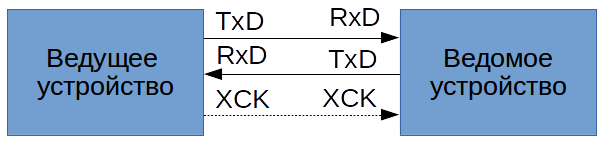
\includegraphics[scale=0.8]{img/usartscheme.png}
	\caption{Схема соединения устройств по интерфейсу USART}
\end{figure}

\textbf{Кадр} ~--- совокупность одного слова данных и сопутствующей информации \cite{usart1}. Начинается кадр со старт-бита, за которым следует младший бит слова данных. Само слово может быть длиной 5-9 битов. После 
старшего бита следует один или два стоп-бита.

\begin{figure}[H]
	\label{usartframe}
	\centering
		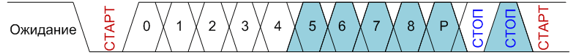
\includegraphics[scale=0.8]{img/usartframe.png}
	\caption{Кадр USART\cite{usart1}}
\end{figure}

В данной работе модуль USART будет использоваться в качестве интерфейса сетевых настроек УСПД, а также для обмена данными с датчиками и счетчиками.

\newpage

\section{Постановка задачи}

Между сервером и клиентом (УСПД) должна происходить передача данных с использованием различных сетевых стандартов. Могут комбинироваться в одном УСПД как проводные, так и беспроводные технологии передачи данных.

На транспортном уровене в стеке протоколов TCP/IP можно использовать протокол UDP, а для прикладного уровня необходимо реализовывать собственный протокол обмена данными. 

Поскольку транспортный протокол должен инкапсулироваться в протоколы нижних уровней, то для начала необходимо построить базис TCP/IP протоколов от физического до транспортного уровня. Следующие разделы будут описывать:
\begin{itemize}
\item физическое соединение УСПД по Ethernet с локальной сетью;
\item построение стека протоколов от канального (Ethernet) до транспортного (UDP);
\item описание и реализация способов конфигурации сетевых настроек УСПД;
\end{itemize}


